\documentclass[11pt,a4paper]{article}

\usepackage[margin=1in]{geometry}
\usepackage[T1]{fontenc}
\usepackage{lmodern}
\usepackage{microtype}
\usepackage{booktabs}
\usepackage{array}
\usepackage{amsmath}
\usepackage{amssymb}
\usepackage{cite}
\usepackage{hyperref}
\usepackage{graphicx}
\usepackage{caption}
\usepackage{xcolor}
\usepackage{placeins}
\usepackage{pgfplots}
\pgfplotsset{compat=1.17}

\hypersetup{colorlinks=true, linkcolor=blue!50!black,
            urlcolor=blue!60!black, citecolor=blue!50!black}

% \bstctlcite from IEEEtran.cls, so the article class can pass options to IEEEtran.bst
\makeatletter
\def\bstctlcite{\@ifnextchar[{\@bstctlcite}{\@bstctlcite[@auxout]}}
\def\@bstctlcite[#1]#2{\@bsphack
  \@for\@citeb:=#2\do{%
    \edef\@citeb{\expandafter\@firstofone\@citeb}%
    \if@filesw\immediate\write\csname #1\endcsname{\string\citation{\@citeb}}\fi}%
  \@esphack}
\makeatother

\newcolumntype{L}[1]{>{\raggedright\arraybackslash}p{#1}}

\title{Entangled Enhancement in a Pipeline of Three ML Components:\\
First Experimental Results}

\author{Ifty Rashedul Arefin}

\date{October 4, 2026}

\begin{document}
\bstctlcite{IEEEexample:BSTcontrol}% no dash for repeated author names

\maketitle

\begin{abstract}
Entangled enhancement is a retraining that improves one component of a
machine learning system (MLS) but fails to improve the whole system, because
the components depend on each other. This report tests entangled enhancement
in a driving pipeline in which all three modules are ML components. The
perception module is updated 30 times on a new city, and every update makes
the perception module more accurate. The prediction module and the planning
module are trained once, either on the ground truth or on the output of the
perception module before the update, and are not retrained after the update.
When the prediction module was trained on the output of the old perception
module, the prediction error increased in 23 of the 30 updates and in 11 of
the 30 updates by more than random variation. When the prediction module was
trained on the ground truth, the prediction error increased by more than
random variation in none of the 30 updates. The planning error changed by at
most 0.13\,m, against a planning error of about 4\,m. None of the measures of
output change that need no ground truth predicted which updates harmed the
prediction module.
\end{abstract}

% ============================================================================
\section{Introduction}
% ============================================================================

An MLS is often built as a pipeline, which is a set of ML components
connected in a line, where each component uses the output of the preceding
component. A component that comes earlier in the line is upstream of a
component that comes later, and the later component is downstream. Retraining
an upstream component can improve that component and still fail to improve
the whole system, because the downstream components depend on the upstream
output. Wang and Machida call this effect entangled enhancement and model when
an MLS should retrain each component~\cite{wang2024compsac,wang2025issre}.
Their models need the probability that retraining the upstream component
leaves the downstream component working, and this probability has not been
measured on a real system.

Earlier experiments in this study used a driving pipeline in which only the
perception module was an ML component, and the prediction module and the
planning module were fixed rules. Fixed rules cannot adapt to the mistakes of
the perception module, and the theory of entangled enhancement explains the
harm by such adaptation. This report replaces the two fixed rules with ML
components and tests whether an update of the perception module can harm the
downstream modules. The report also tests whether a sign that needs no ground
truth can show which updates cause the harm.

This report makes three contributions. First, the report describes a pipeline of three
ML components that is trained and tested on a reduced nuScenes dataset, with
the prediction module and the planning module checked against simple
baselines. Second, the report gives the results of 30 updates of the perception module and counts
the updates in which the prediction error or the planning error increased by
more than random variation. Third, the report shows how well nine measures of output
change, which need no ground truth, separate harmful updates from harmless
updates.

% ============================================================================
\section{Background}
\label{sec:background}
% ============================================================================

This section defines the pipeline, the error measures and the two possible
causes of entangled enhancement. Every later section uses these definitions.
The pipeline and the data are the same as in the earlier experiments of this
study, and the error measures are the standard measures for prediction and
planning on nuScenes.

\paragraph{Pipeline:} The ego vehicle is the vehicle that the pipeline drives.
The perception module $C_1$ (YOLOv11n~\cite{jocher2024yolo11}) finds the
objects around the ego vehicle in the image of the front camera. The
prediction module $C_2$ predicts where each object will move over the next
3\,s. The planning module $C_3$ chooses the path that the ego vehicle will
drive over the next 3\,s, which we call the planned path. The data come from
nuScenes~\cite{caesar2020nuscenes}, which is divided into scenes of about
20\,s recorded in Boston and Singapore. The correct position of every object is
labelled by hand, and we call these labelled values the ground truth.

\paragraph{Updates and error measures:} An update is one retraining of $C_1$
on Singapore images, starting from the $C_1$ that was trained in Boston. We
call $C_1$ before an update the old $C_1$ and $C_1$ after the update the new
$C_1$. We write $\delta_1$ for the gain in mAP50 of $C_1$, the standard
accuracy measure for object detection. The prediction error is the minADE,
which is the average distance between the predicted path and the true path
of an object, taken for the best of the six paths that $C_2$ predicts. The
planning error is the distance between the planned path and the path of the
human driver at 3\,s. We write $\Delta_2$ and $\Delta_3$ for the increase of
the prediction error and of the planning error after an update.

\paragraph{Causes of entangled enhancement:} An update shows entangled
enhancement when $\delta_1 > 0$ and $\Delta_2 > 0$ or $\Delta_3 > 0$. The
harm can have two causes. In the first cause, the downstream modules adapted
during training to the mistakes of the old $C_1$ and are disturbed when those
mistakes change. In the second cause, $C_1$ improves on average but becomes
worse on the cases that matter downstream. The first cause can act only when
the downstream modules were trained on the output of the old $C_1$, and this
condition is the basis of the comparison in Section~\ref{sec:setup}.

% ============================================================================
\section{Hypotheses}
% ============================================================================

This section states the two hypotheses that the experiment tests. The first
hypothesis concerns whether entangled enhancement occurs in a pipeline of
three ML components. The second hypothesis concerns a symptom of entangled
enhancement. A symptom is a sign that an update harms the downstream modules,
measured without ground truth.

\paragraph{H1 (existence):} In a pipeline in which all three modules are ML
components, an update of $C_1$ can increase the prediction error or the
planning error, even when the update makes $C_1$ more accurate. H1 does not
claim that every update causes harm. H1 claims that a clear number of updates
cause an increase that is larger than random variation. H1 also claims that
the increase is larger when the downstream modules were trained on the output
of the old $C_1$.

\paragraph{H2 (symptom):} The change in the output of $C_1$ and of $C_2$
after an update, measured on the same test images without ground truth, is
larger in the updates that harm the downstream modules than in the other
updates. The gain $\delta_1$ alone does not separate the two groups of
updates. If H2 holds, an engineer who maintains the MLS can compute the change
before using an update and retrain the downstream modules when the change is
large.

% ============================================================================
\section{Experimental Setup}
\label{sec:setup}
% ============================================================================

This section describes the data, the 30 updates of $C_1$, the ML models for
$C_2$ and $C_3$, the two ways of training $C_2$ and $C_3$, and the threshold
for random variation. All training and testing ran on one Tesla T4 graphics
card on Kaggle. Every trained model was saved and reused, and no model was
trained twice.

\subsection{Dataset}

The experiment uses 350 of the 850 scenes of nuScenes, with the full-size
images of the front camera only, which reduces the data from 45\,GB to
4.6\,GB. Table~\ref{tab:data} lists the four parts of the dataset. Boston is
split into two separate parts, one to train $C_1$ and one to train $C_2$ and
$C_3$. A perception module is much more accurate on the scenes used to train
that perception module~\cite{xu2024realworld}, and $C_2$ and $C_3$ must learn
from the realistic mistakes of $C_1$. One scene in seven of the Boston part
for $C_2$ and $C_3$ is kept apart as a validation set. The validation set
decides when to stop training, before the models overfit.

\begin{table}[h!]
\centering
\caption{The four parts of the reduced dataset}
\label{tab:data}
\small
\renewcommand{\arraystretch}{1.25}
\begin{tabular}{@{}lccL{6.0cm}@{}}
\toprule
\textbf{Part} & \textbf{Scenes} & \textbf{Images} & \textbf{Used for} \\
\midrule
Boston 1    & 100 & 4{,}008 & training the old $C_1$ \\
Boston 2    & 100 & 4{,}046 & training $C_2$ and $C_3$ (86 scenes) and validation (14 scenes) \\
Singapore 1 & 100 & 3{,}997 & updating $C_1$ \\
Singapore 2 &  50 & 2{,}020 & testing every module \\
\bottomrule
\end{tabular}
\end{table}

\subsection{Updates of the Perception Module}

The old $C_1$ was trained on Boston 1 twice, with the random seeds 0 and 1. A
random seed is the starting number for the random choices made during
training, and two seeds give two slightly different models. The two old
$C_1$ reach an mAP50 of 0.109 and 0.117 on the test part. Each update starts
from one old $C_1$ and retrains on Singapore 1 with one of the 15 settings
in Table~\ref{tab:updates}. The 15 settings applied to both old $C_1$ give 30
updates.

\begin{table}[h!]
\centering
\caption{The 15 settings of an update of $C_1$, applied to both old $C_1$}
\label{tab:updates}
\small
\renewcommand{\arraystretch}{1.25}
\begin{tabular}{@{}lccc@{}}
\toprule
\textbf{Group} & \textbf{Share of Singapore 1} & \textbf{Training passes} & \textbf{Seeds} \\
\midrule
Data size & 100\,\%, 50\,\%, 25\,\% (3{,}575, 1{,}788, 894 images) & 10 & 1, 2, 3 \\
Training length & 100\,\% & 5, 20 & 1, 2, 3 \\
\bottomrule
\end{tabular}
\end{table}

\subsection{Prediction and Planning Modules}

$C_2$ follows AutoBot-Ego~\cite{girgis2022autobots}. For every object found by
$C_1$, the model describes each object of the last four keyframes relative to
that object, and a transformer learns which earlier objects are the same
object~\cite{weng2022whose}. No hand-written tracker links the objects across
images. $C_3$ follows PlanT~\cite{renz2022plant}, with one input token per
object, a token for the driving command (left, straight or right) and a
recurrent decoder that outputs six points of the planned path. Both models
were trained with early stopping on the validation scenes.

A planning module that receives the speed of the ego vehicle can score well on
nuScenes while the planning module ignores the
objects~\cite{zhai2023rethinking,li2024egostatus}. We therefore trained $C_3$
in two variants, without any ego input and with the positions of the ego
vehicle over the last 1.5\,s. Table~\ref{tab:validity} compares both variants
with two simple baselines on the test part. The variant without ego input does
not beat the baseline that drives the average Boston path for each command,
and the experiment uses the variant with the ego path.

\begin{table}[h!]
\centering
\caption{$C_2$ and $C_3$ against simple baselines on the test part}
\label{tab:validity}
\small
\renewcommand{\arraystretch}{1.25}
\begin{tabular}{@{}L{5.4cm}L{3.3cm}L{4.6cm}@{}}
\toprule
\textbf{Model and input} & \textbf{Error} & \textbf{Baseline} \\
\midrule
$C_2$ on ground truth & 0.77\,m & 4.48\,m (each object stays still) \\
$C_2$ on the output of $C_1$ & 2.39 to 2.95\,m & 5.39 to 5.85\,m (each object stays still) \\
$C_3$ without ego input & 9.3 to 12.5\,m & 9.25\,m (average path per command) \\
$C_3$ with the ego path & 3.70 to 4.16\,m & 9.25\,m (average path per command) \\
\bottomrule
\end{tabular}
\end{table}

The variant with the ego path still uses the objects. When the objects are
removed from the input of $C_3$, the planned position at 3\,s moves by 0.73 to
1.65\,m on average, which is above the threshold of 0.5\,m set before the
experiment. The collision rate is the fraction of test samples in which the planned path
overlaps an object. The collision rate is 0.05 to 0.08 for this variant and
0.18 for the baseline.

\subsection{Training of the Prediction and Planning Modules}

The first cause in Section~\ref{sec:background} can act only when $C_2$ and
$C_3$ were trained on the output of the old $C_1$. We therefore train $C_2$
and $C_3$ in two ways and keep both fixed during all 30 updates. In the first
way, $C_2$ and $C_3$ learn from the ground truth and have never seen a
mistake of $C_1$. In the second way, $C_2$ and $C_3$ learn from the output of
the old $C_1$ that the update starts from. After training, both versions run
in the normal pipeline, with the output of $C_1$ as the input of $C_2$.

\subsection{Random Variation}

A change counts as harm only when the change is larger than random variation.
We measure random variation by replacing the old $C_1$ with the other old
$C_1$, which differs only in the random seed. The largest change caused by
this replacement is 0.112\,m in prediction error and 0.018\,m in planning
error. An update is counted as harmful when $\Delta_2 > 0.112$\,m or
$\Delta_3 > 0.018$\,m. The outputs of $C_2$ and $C_3$ on the ground truth were
checked before and after every update. The outputs stayed exactly the same,
which confirms that only the output of $C_1$ changed.

% ============================================================================
\section{Results}
% ============================================================================

This section reports the effect of the 30 updates on $C_2$ and on $C_3$, the
comparison with $C_2$ and $C_3$ retrained on the new $C_1$, and the test of
the symptom. Every update made $C_1$ more accurate, with $\delta_1$ between
0.048 and 0.118 in mAP50. The new $C_1$ reach an mAP50 between 0.166 and
0.235, against 0.109 and 0.117 for the two old $C_1$.

\subsection{Effect on the Prediction Module}

Figure~\ref{fig:delta2} shows $\Delta_2$ for every update and both ways of
training. The $C_2$ trained on the output of the old $C_1$ has a larger
$\Delta_2$ than the $C_2$ trained on the ground truth in all 30 updates. The
difference is largest for the updates that start from the old $C_1$ with seed
0, where $\Delta_2$ lies between $+0.049$ and $+0.284$\,m, with a mean of
$+0.165$\,m. For the updates that start from the old $C_1$ with seed 1, the
mean $\Delta_2$ is $-0.008$\,m.

\begin{figure}[htbp]
\centering
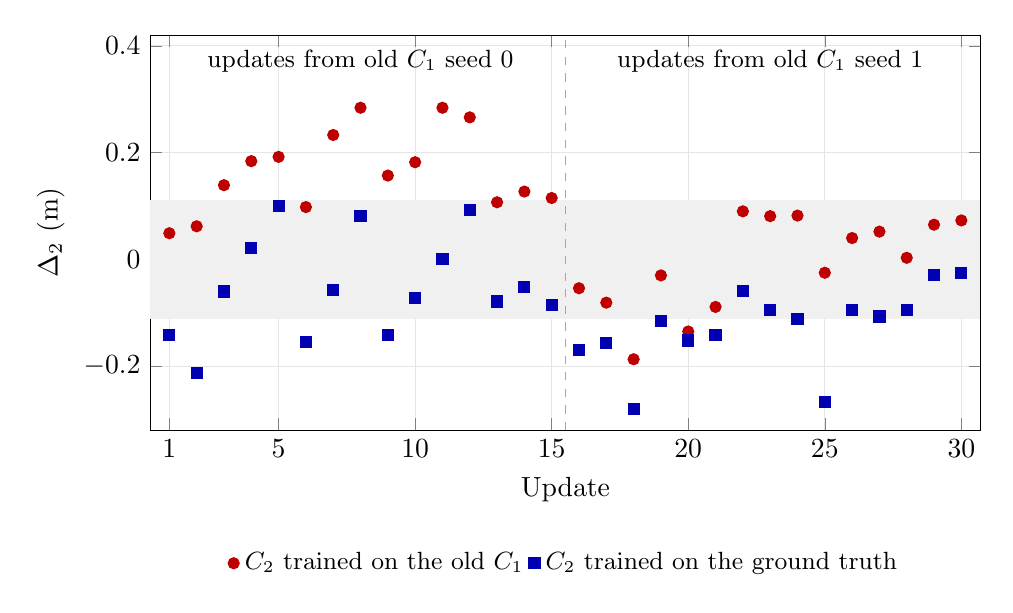
\begin{tikzpicture}
\begin{axis}[width=\textwidth, height=6.6cm,
    xlabel={Update}, ylabel={$\Delta_2$ (m)},
    xmin=0.3, xmax=30.7, ymin=-0.32, ymax=0.42,
    xtick={1,5,10,15,20,25,30},
    legend style={at={(0.5,-0.28)}, anchor=north, legend columns=2, font=\small, draw=none},
    grid=major, grid style={gray!20}]
\fill[gray!12] (axis cs:0.3,-0.112) rectangle (axis cs:30.7,0.112);
\draw[gray!70, dashed] (axis cs:15.5,-0.32) -- (axis cs:15.5,0.42);
\addplot[only marks, mark=*, color=red!75!black] coordinates {
(1,0.049) (2,0.062) (3,0.139) (4,0.184) (5,0.192) (6,0.098) (7,0.233) (8,0.284) (9,0.157) (10,0.182) (11,0.284) (12,0.266) (13,0.107) (14,0.127) (15,0.115) (16,-0.054) (17,-0.081) (18,-0.187) (19,-0.030) (20,-0.135) (21,-0.089) (22,0.090) (23,0.081) (24,0.082) (25,-0.025) (26,0.040) (27,0.052) (28,0.003) (29,0.065) (30,0.073)};
\addlegendentry{$C_2$ trained on the old $C_1$}
\addplot[only marks, mark=square*, color=blue!70!black] coordinates {
(1,-0.141) (2,-0.212) (3,-0.060) (4,0.021) (5,0.100) (6,-0.154) (7,-0.058) (8,0.082) (9,-0.141) (10,-0.073) (11,0.001) (12,0.093) (13,-0.079) (14,-0.051) (15,-0.085) (16,-0.170) (17,-0.156) (18,-0.280) (19,-0.115) (20,-0.152) (21,-0.141) (22,-0.059) (23,-0.095) (24,-0.111) (25,-0.267) (26,-0.094) (27,-0.107) (28,-0.094) (29,-0.029) (30,-0.025)};
\addlegendentry{$C_2$ trained on the ground truth}
\node[font=\small, anchor=north] at (axis cs:8,0.41) {updates from old $C_1$ seed 0};
\node[font=\small, anchor=north] at (axis cs:23,0.41) {updates from old $C_1$ seed 1};
\end{axis}
\end{tikzpicture}
\caption{Increase of the prediction error $\Delta_2$ in the 30 updates (grey band: random variation)}
\label{fig:delta2}
\end{figure}

Table~\ref{tab:counts} counts the updates with an increase. Counted above
random variation, the prediction error increased in 11 of the 30 updates for
the $C_2$ trained on the output of the old $C_1$, and all 11 updates start
from the old $C_1$ with seed 0. For the $C_2$ trained on the ground truth, no
update increased the prediction error by more than random variation. The
contrast shows the first cause, because only the $C_2$ that adapted to the
old $C_1$ was harmed.

\begin{table}[h!]
\centering
\caption{Number of updates, out of 30, in which the error increased}
\label{tab:counts}
\small
\renewcommand{\arraystretch}{1.25}
\begin{tabular}{@{}L{5.6cm}cccc@{}}
\toprule
& \multicolumn{2}{c}{\textbf{Any increase}} & \multicolumn{2}{c}{\textbf{Above random variation}} \\
\cmidrule(lr){2-3}\cmidrule(l){4-5}
\textbf{$C_2$ and $C_3$ trained on} & $\Delta_2 > 0$ & $\Delta_3 > 0$ & $\Delta_2 > 0.112$\,m & $\Delta_3 > 0.018$\,m \\
\midrule
the output of the old $C_1$ & 23 & 18 & 11 & 13 \\
the ground truth & 5 & 29 & 0 & 29 \\
\bottomrule
\end{tabular}
\end{table}

\subsection{Effect on the Planning Module}

The planning error increased by more than random variation in 13 of the 30
updates for the $C_3$ trained on the output of the old $C_1$. The same
increase appears in 29 of the 30 updates for the $C_3$ trained on the ground
truth, and the first cause cannot explain an increase in that case. All
changes of the planning error are small, with a mean $\Delta_3$ between
$-0.006$ and $+0.058$\,m and a largest value of 0.13\,m, against a planning
error of about 4\,m. In 21 of the 30 updates, the prediction error or the
planning error increased by more than random variation for the modules trained
on the output of the old $C_1$.

\subsection{Retraining on the New Perception Module}

Two further updates, one from each old $C_1$ with all of Singapore 1 and 10
training passes, were used to retrain $C_2$ and $C_3$ on the output of the new
$C_1$. Retraining removes the old mistakes from the training data. After the
update, the $C_2$ trained on the old $C_1$ has a prediction error of 2.75 and
2.61\,m, and the retrained $C_2$ has 2.39 and 2.45\,m. The $C_3$ trained on
the old $C_1$ has a planning error of 4.14 and 4.00\,m, and the retrained
$C_3$ has 3.71 and 3.70\,m. Retraining the downstream modules together with
$C_1$ gave lower errors in both updates. Two updates are too few for a general
statement.

\subsection{Test of the Symptom}

For each update we computed nine measures of output change on the test images
without ground truth. Seven measures compare the output of $C_1$ before and
after the update, for example the mix of object types and the confidence
scores, and two measures compare the predicted paths of $C_2$.
Table~\ref{tab:h2} gives the rank correlation (Spearman) between each measure
and $\Delta_2$, which is close to 1 when a larger measure always comes with a
larger $\Delta_2$. The table also gives the AUROC, which is the probability
that a harmful update ($\Delta_2 > 0$) has a larger measure than a harmless
update.

\begin{table}[h!]
\centering
\caption{Measures of output change against $\Delta_2$ (trained on the old $C_1$)}
\label{tab:h2}
\small
\renewcommand{\arraystretch}{1.2}
\begin{tabular}{@{}L{6.6cm}cccc@{}}
\toprule
& \multicolumn{2}{c}{\textbf{All 30 updates}} & \multicolumn{2}{c}{\textbf{Rank correlation per old $C_1$}} \\
\cmidrule(lr){2-3}\cmidrule(l){4-5}
\textbf{Measure} & \textbf{Rank corr.} & \textbf{AUROC} & \textbf{Seed 0} & \textbf{Seed 1} \\
\midrule
$\delta_1$ (needs ground truth) & $+0.04$ & 0.66 & $-0.03$ & $-0.01$ \\
$C_1$: objects per image (Jensen--Shannon) & $-0.01$ & 0.32 & $+0.58$ & $-0.14$ \\
$C_1$: mix of object types (Jensen--Shannon) & $-0.51$ & 0.26 & $-0.26$ & $-0.20$ \\
$C_1$: confidence (Wasserstein) & $-0.29$ & 0.46 & $-0.45$ & $-0.10$ \\
$C_1$: confidence (Kolmogorov--Smirnov) & $-0.21$ & 0.52 & $-0.56$ & $-0.09$ \\
$C_1$: forward position (Wasserstein) & $+0.13$ & 0.63 & $-0.19$ & $+0.25$ \\
$C_1$: lateral position (Wasserstein) & $+0.26$ & 0.68 & $-0.16$ & $+0.17$ \\
$C_1$: objects found by one version only & $-0.02$ & 0.58 & $-0.10$ & $-0.04$ \\
$C_2$: predicted movement (Wasserstein) & $+0.02$ & 0.60 & $+0.13$ & $+0.08$ \\
$C_2$: shift of the predicted position & $+0.68$ & 0.81 & $+0.29$ & $-0.28$ \\
\bottomrule
\end{tabular}
\end{table}

The shift of the predicted position of the same object has the highest rank
correlation over all 30 updates ($+0.68$, AUROC 0.81). For each old $C_1$
separately, however, the rank correlation is $+0.29$ and $-0.28$. The high
value over all updates comes from the difference between the two old $C_1$,
because the updates from seed 0 have both larger shifts and a larger
$\Delta_2$. No measure separates harmful and harmless updates consistently for
both old $C_1$, and H2 is not supported by the present data.

% ============================================================================
\section{Discussion}
% ============================================================================

This section discusses three limits of the results. The limits concern the
threshold for random variation, the number of pipelines, and the small role of
the objects in the planning module. Each limit points to a further experiment
that can strengthen or weaken the conclusion.

\paragraph{Threshold for random variation:} The threshold comes from one
replacement of the old $C_1$ by the other old $C_1$ for each starting point. A
paired bootstrap over the 50 test scenes would give an interval for every
single update and a firmer count. The difference between the two old $C_1$ is
also large, with 11 of 15 harmful updates for seed 0 and none for seed 1.
More old $C_1$ trained with other seeds are needed to show how often a
starting point leads to harm.

\paragraph{One pipeline:} All results come from one choice of models,
AutoBot-Ego for $C_2$ and PlanT for $C_3$. Entangled enhancement may depend on
this choice. The same test with Social-LSTM~\cite{alahi2016social} for $C_2$
and AD-MLP~\cite{zhai2023rethinking} for $C_3$, in the four combinations of
the two models for each module, can show whether the effect occurs in every
pipeline.

\paragraph{Role of the objects in planning:} The variant of $C_3$ with the
ego path beats the baselines, but the objects move the planned position by
only 0.73 to 1.65\,m. A planning module that depends little on the objects
can be affected little by $C_1$, which may explain the small values of
$\Delta_3$. A planning module that depends more on the objects is needed to
measure the effect of $C_1$ on planning with more power.

% ============================================================================
\section{Conclusion}
% ============================================================================

This report tested entangled enhancement in a pipeline of three ML components
with 30 updates of the perception module, all of which made the perception
module more accurate. The prediction module trained on the output of the old
perception module became worse by more than random variation in 11 of the 30
updates, and the prediction module trained on the ground truth in none. This
result supports H1 for the prediction module and points to the first cause,
the adaptation of the downstream module to the mistakes of the old perception
module.

The planning module changed by at most 0.13\,m, and the increase also appeared
when the planning module was trained on the ground truth. None of the nine
measures of output change predicted the harm consistently, and H2 is not
supported. The next experiments are a paired bootstrap for every update, more
old perception modules with other seeds, retraining on the new perception
module for more updates, and the three other pipelines.

\FloatBarrier
\bibliographystyle{IEEEtran}
\bibliography{references}

\end{document}
